\chapter{Detail Design}

\section{Relay Switch Circuit}

As explained in section \ref{sec:relay-switch}, a relay switch (the Mantech NT72C 12V DC relay
[\cite{manual:relay-specs}]), in conjunction with a 2N2222 Bipolar Junction Transistor (BTJ)
[\cite{manual:transistor-datasheet}], is used by the Raspberry Pi to switch the motor on and
off. See Figure \ref{fig:relay-switch} for the circuit diagram.

\begin{figure}[h]
\centering
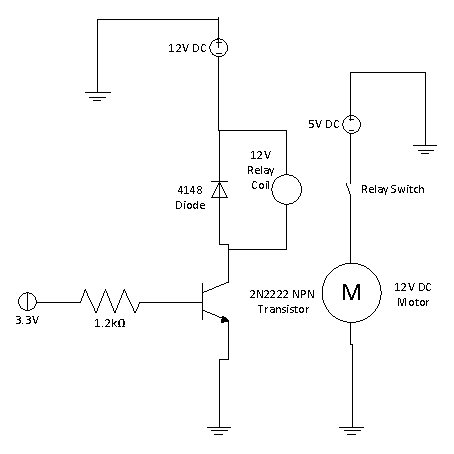
\includegraphics[scale=0.7]{relay_switch.eps}
\caption{12V relay transistor switch. }
\label{fig:relay-switch}
\end{figure}

The relevant  parameters for these components are [\cite{manual:relay-specs},
\cite{manual:transistor-datasheet}]:

\[ P_{r} = 0.36W\]
\[ V_{r} = 12V\]
\[ \beta \approx 10\]
\[ V_{p} = 3.3V\]

From the relays power dissipation and voltage, its current draw is found by

\[
I_{r} = \frac{P_{r}}{V_{r}}
\]

which gives a current draw of

\[
I_{r} = 0.03A
\]

Taking the BJT's current amplification as roughly 10, the current draw from the Pi to the
base of the BJT is given by

\[
I_{b} = \frac{I_{r}}{\beta} = \frac{I_{c}}{\beta}
\]

This gives a current draw of

\[
I_{b} = 0.003A = 3mA
\]

The maximum current draw from the GPIO pins is 16mA [\cite{website:gpio-specs}], though this is
not recommended as the Pi does not have any current limiting or over-current protection.
Therefore, a current draw of 3 mA is completely safe.

To limit the current draw from the Pi, a base resistor must be added between the Pi's GPIO pin
and the BJT's base. With a current draw of $3mA$ and a voltage of $3.3V$, the resistor size is
found by Ohm's law as follows

\[
R_{b} = \frac{V_{p}}{I_{p}}
\]

which gives

\[
R_{b} = 1.1k\Omega
\]

Compensating for tolerances by adding 10\%, the resistor size is set to

\[R_{b} = 1.2k\Omega\]

which draws a current of 

\[I_{b} = 2.75 mA \]

which is still within the acceptable range.

\section{Security Scheme}
\label{sec:security-code-scheme}

In addition to the assymetric encryption used on all data transfer to and from
the server to its clients, two more layers of security were added to prevent
repeated use of the same code and to make it harder for hackers to crack the
encryption key.

\subsection{Random Character String}

The product code transmitted to the server is embedded inside a
random 16-character string of hex values, i.e. numbers from 1 to 9 or characters
from A to F. The product code is a 4 character hex string, but this is saved on
the database and can therefore not be random. 

This is done to prevent any would-be
hackers from realising that they have cracked the system's encryption. In other
words, if the hackers have cracked the encryption, they will still see 16
random hex characters and think that the encryption is still intact.

\subsection{Challenge and Response Code}

The second layer of security added is a challenge/response system. Such a system
works by having party A generate a challenge (this can be a string or a number).
Party B then takes this challenge and puts it through a previosuly agreed-upon
process, e.g. makes the letters capital or adds the numbers together. This
is the response. Party B then sends the back the response to party A, which then
checks to see if its a valid response to party A's original challenge.

In the case of the vending machine, a 16 character hex string is being
generated. It was decided to use 4 characters of this random string as the
vending machine's challenge. After receiving this challenge, the server then
takes out the agreed-upon 4 characters and adds it to the server's response
code. When the vending machine scans the customer's response QR Code, the
vending machine checks to see if the 4 character response was part of its
original code the vending machine generated.

This system is used to prevent customers from only buying one product and using
the same code again to get another product for free. Thus, the
challenge/response code system makes each code only valid for one transaction.

\section{Web Server Program Design}

The web server that was made for this project is based on the Django web framework for Python
(see Section \ref{sec:django} for some background information). The Django server was then
configured to run on top of an Apache web server located on an Amazon Web Service (AWS) Elastic
Compute Cloud (EC2) cloud computer instance (see Section \ref{sec:ec2} for some background
on EC2 and Section \ref{sec:apache} for some background on Apache).

The server is responsible for handling all the data and financial transactions that will take
place during the vending machine's operation. 

This section stipulates the design of the complete server and how the different components
interact with one another. 

\subsection{Django Server}

The Django server is responsible for all of the scripting and database work that the server
performs. The server is divided up into a total of six applications. Each of these is
responsible for either displaying a single web page or to handle data requests from the
Near Field Communication (NFC) Android app (see Section \ref{sec:nfc-android-app} for more
details).

The website apps and their interactions with the real world and one another
are given in Figure \ref{fig:website-apps}. 

\begin{figure}[h]
 \centering 
 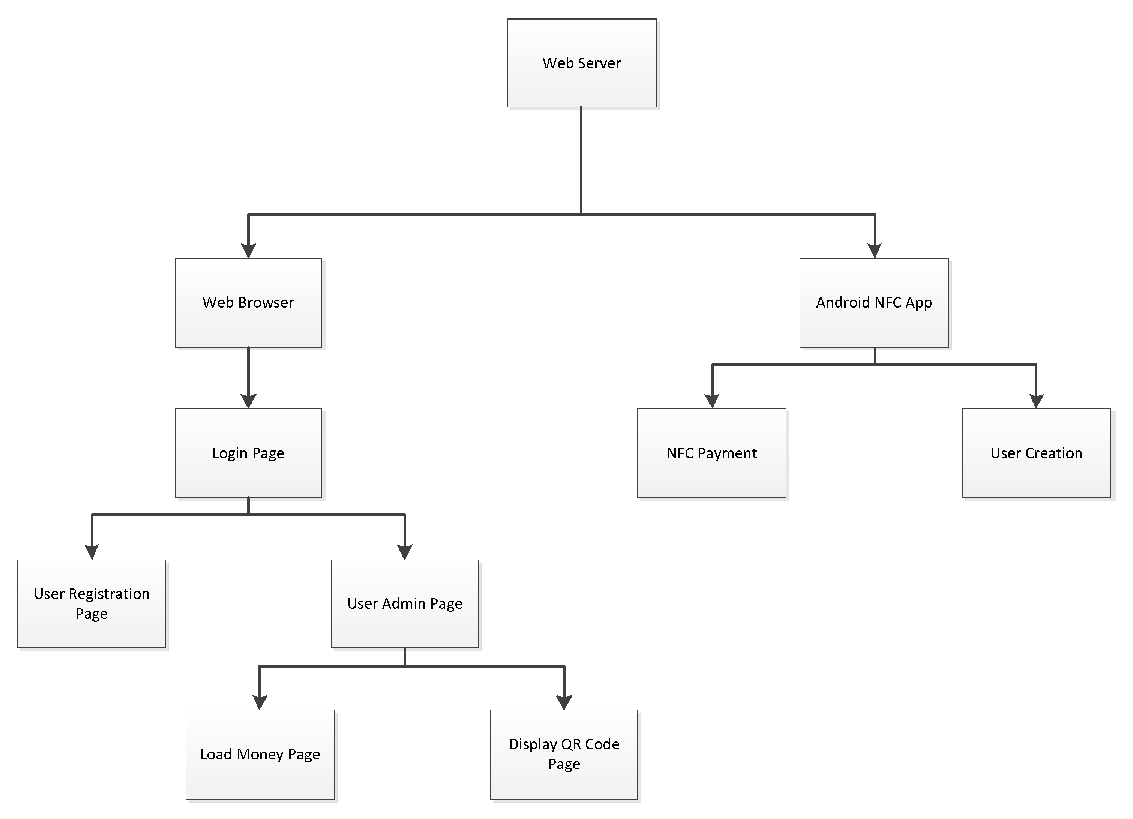
\includegraphics[clip=true, trim = 0 130 130 30,
 scale=0.7]{website_structure}
 \caption{The web server app structure}
 \label{fig:website-apps}
\end{figure}

\subsubsection{display\_qrcode}

This app forms the core of the Quick Response Code (QR Code) payment handling part of the
server. See Figure \ref{fig:disp-qrcode} for the process flow of this app.

\begin{figure}[h]
 \centering 
 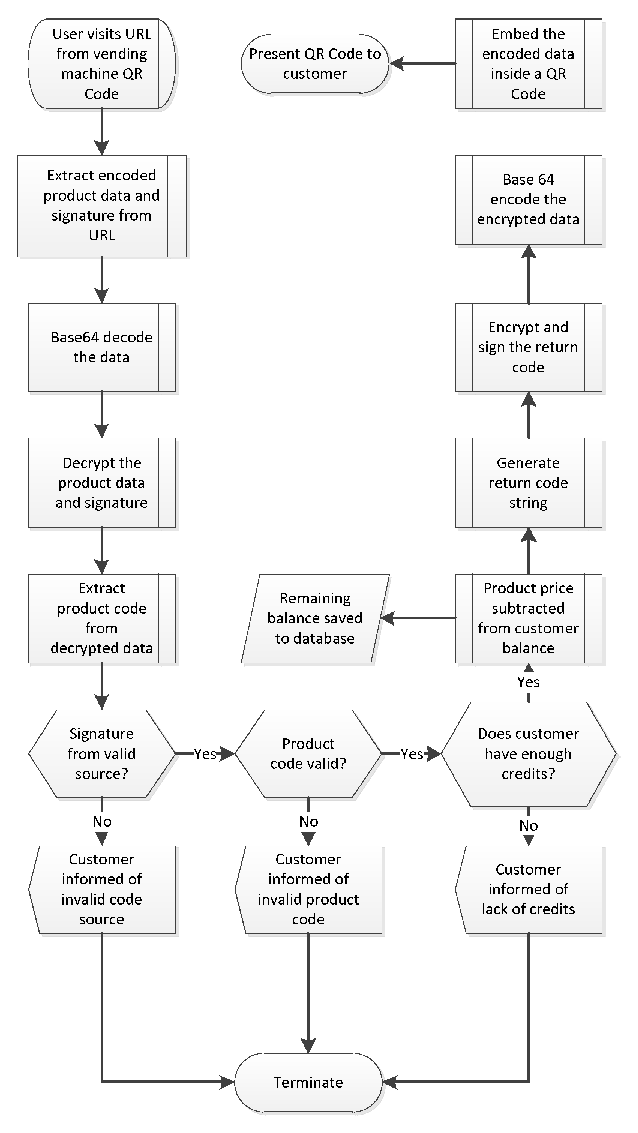
\includegraphics[clip=true, trim = 0 250 0 50,
 scale=0.7]{qrcode_processflow_server_bak}
 \caption{The display\_qrcode app processflow}
 \label{fig:disp-qrcode}
\end{figure}

As seen from Figure \ref{fig:disp-qrcode}, the app first extracts the code containing the
product code and vending machine's signature from the Uniform Resource Locator (URL) that the
customer visited with his/her cell phone's web browser. The app then proceeds to decode the
the code from the base64 encoded format it was sent in (see Section \ref{sec:base64} for some
background information on base 64 encoding).

After successfully decoding the data, the app proceeds to decrypt the data and signature with the ElGamal
algorithm using the server's private key and the vending machine's public key
(see Section \ref{sec:assymetric-encryption} for more detail on public and private keys) and, following the
security code scheme described in Section \ref{sec:security-code-scheme}, extracts the product
code from the decrypted string.

The app then checks to see if the signature comes from a valid source (i.e. one of the vending
machines using this system), if the product code is valid (i.e. the product is in the database)
and if the customer has enough credits loaded loaded onto his/her account. If either of these
checks return false, an appropriate error message is shown to the customer explaining what
went wrong and what the customer should do next.

If the checks were passed, the app proceeds to subtract the product cost from the user's
remaining balance. Using the security code scheme, the app then generates the correct return
code, encrypts and signs it with the vending machine's public key and the server's private key,
and encodes it with base 64. After this is completed, the app embeds this data into a QR Code,
which is returned to the customer's cell phone screen. 

\subsubsection{load\_money}

This app allows the customer to load money onto his/her account. At the moment it makes use of
faux money, meaning that the money loaded has no real-world value. The customer can load a
maximum of R1000.00 onto his/her account.

See Figure \ref{fig:load-money} for the process flow of this app.

\begin{figure}[h]
 \centering 
 \includegraphics[clip=true, trim = 0 580 100 60,
 scale=0.7]{load_money}
 \caption{The load\_money app process flow}
 \label{fig:load-money}
\end{figure}

\subsubsection{nfc}

This app forms the core of the NFC payment handling part of the server. See Figure
\ref{fig:nfc-process} for a detailed process flow diagram.

\begin{figure}[h]
 \centering 
 \includegraphics[clip=true, trim = 0 200 100 80,
 scale=0.7]{nfc_processflow_bak}
 \caption{The nfc app process flow}
 \label{fig:nfc-process}
\end{figure}

As seen from Figure \ref{fig:nfc-process}, the server first extracts the encoded and encrypted
customer login details and product code from the URL the NFC app sends to the server. These
codes are then all decoded and decrypted using the Ron Rivest, Adi Shamir and Leonard Adleman
(RSA) algorithm and the server's private key. 

The user login details are then checked and verified using the server's user database. If this
check fails, the customer is given an appropriate error message and informed to create a user
profile. 

If the check is passed, the server then checks to see if the customer has enough money loaded
onto his/her account. If this check fails, the customer is informed of his/her lack of funds
and is instructed to load more money. If the check is passed, the server subtracts the product
cost from the customer's balance and encrypts and encodes a confirmation code, according to the
security code scheme spesified in Section \ref{sec:security-code-scheme}, which is then sent
to the NFC app. 

\subsubsection{nfc\_add\_user}

This app allows a customer using the NFC app to create a user profile for himself/herself. The
server extracts the customer's login details from the URL request that the NFC app send to the
server. The user name and email are kept in plain text, but the password is decrypted to
plain text with the RSA algorithm and the server's private key.

These details are then saved to the database and is immediately available to be used by the new
customer. 

\subsubsection{register}

This app allows a new customer to register. This app is only accessible by a web browser and
not by the NFC app. However, a user registered with this app will be able to use the same login
details for the NFC app.

The app presents the user with a simple registration page which asks for a user name, email and
password. Using Django's built-in form support. This allows the server to handle the
POST request that is generated when the customer presses the `Continue' button. When this is
done, the login data contained within the POST request is extracted and saved into the user
database. 

\subsection{EC2}

The AWS EC2 server provides the platform on which the Apache server runs. The EC2 server
instance was configured to run Ubuntu 12.10, `Quantal Quetzal'. This was done because most of
the server development was done on Ubuntu 12.10, and the server code will therefore require
minimal adaptation to be able to run on the EC2 server. 

After the server instance was created, the following packages and programs were installed for
the server to be able to run properly:

\begin{itemize}
  \item Apache2: Installs the Apache server framework.
  \item libapache2-mod-wsgi: An Apache module that allows Apache to work with Python wsgi
  scripts.
  \item python-pip: Allows Ubuntu to install Django from the Python Package Index (PyPI)
  [\cite{website:pypi}].
  \item Django: Installs the all the Django packages that will be used by the server. 
\end{itemize}

Because the server's database uses SQLite3, and Ubuntu 12.10 comes with it by default, no
external database programs were needed to be installed. 

After this was completed, the server is fully capable of serving Django webpages. 

\subsection{Apache}

The Apache server framework provides the foundation on which the Django server runs. It had to
be configured to be able to run the Python scripts that Django contains. To do this, the steps
described in Nick Polet's blog post was followed [\cite{article:apache-setup}]. It describes
in detail how to configure Apache to serve a Django website.

For Apache to be able to serve Django sites, it had to be configured to run the Web Server
Gateway Interface (wsgi.py) script located within the Django server folder. This was done by
adding the following code to the Apache's httpd.conf configuration file:

\begin{verbatim}
WSGIScriptAlias / /home/ubuntu/srv/server_site/server_site/wsgi.py
WSGIPythonPath /home/ubuntu/srv/server_site

<Directory /home/ubuntu/srv/server_site/server_site>
<Files wsgi.py>
Order deny,allow
Allow from all
</Files>
</Directory>
\end{verbatim}

The following line was also needed to be added to Apache's apache2.conf file:

\begin{verbatim}
Include httpd.conf
\end{verbatim}

\section{Vending Program}

The vending machine's program runs the vending machine. Its responsible for
allowing the cuustomer to select a product, to create a QR Code for that points
takes the customer to the web server, to scan the customer's response QR Code,
to scan the customer's NFC request and to dispense the product after a
successful transaction. The whole program is based on Python scripts and
designed to be used by a Raspberry Pi microcomputer (see Section
\ref{sec:raspi} for more details).

To simplify the program, its split up into separate sub-programs. These
sub-programs, called scripts, are discussed in this section.

\subsection{User Interface}

To allow the customer to select a product, a Graphical User Interface (GUI) was
created. The GUI was made using the WX Python GUI toolkit
[\cite{website:wx-python}].
See Figure \ref{fig:gui-screenshot} for a screenshot of the GUI and Figure
\ref{fig:gui-processflow} for the GUI process flow.

\begin{figure}[h]
 \centering 
 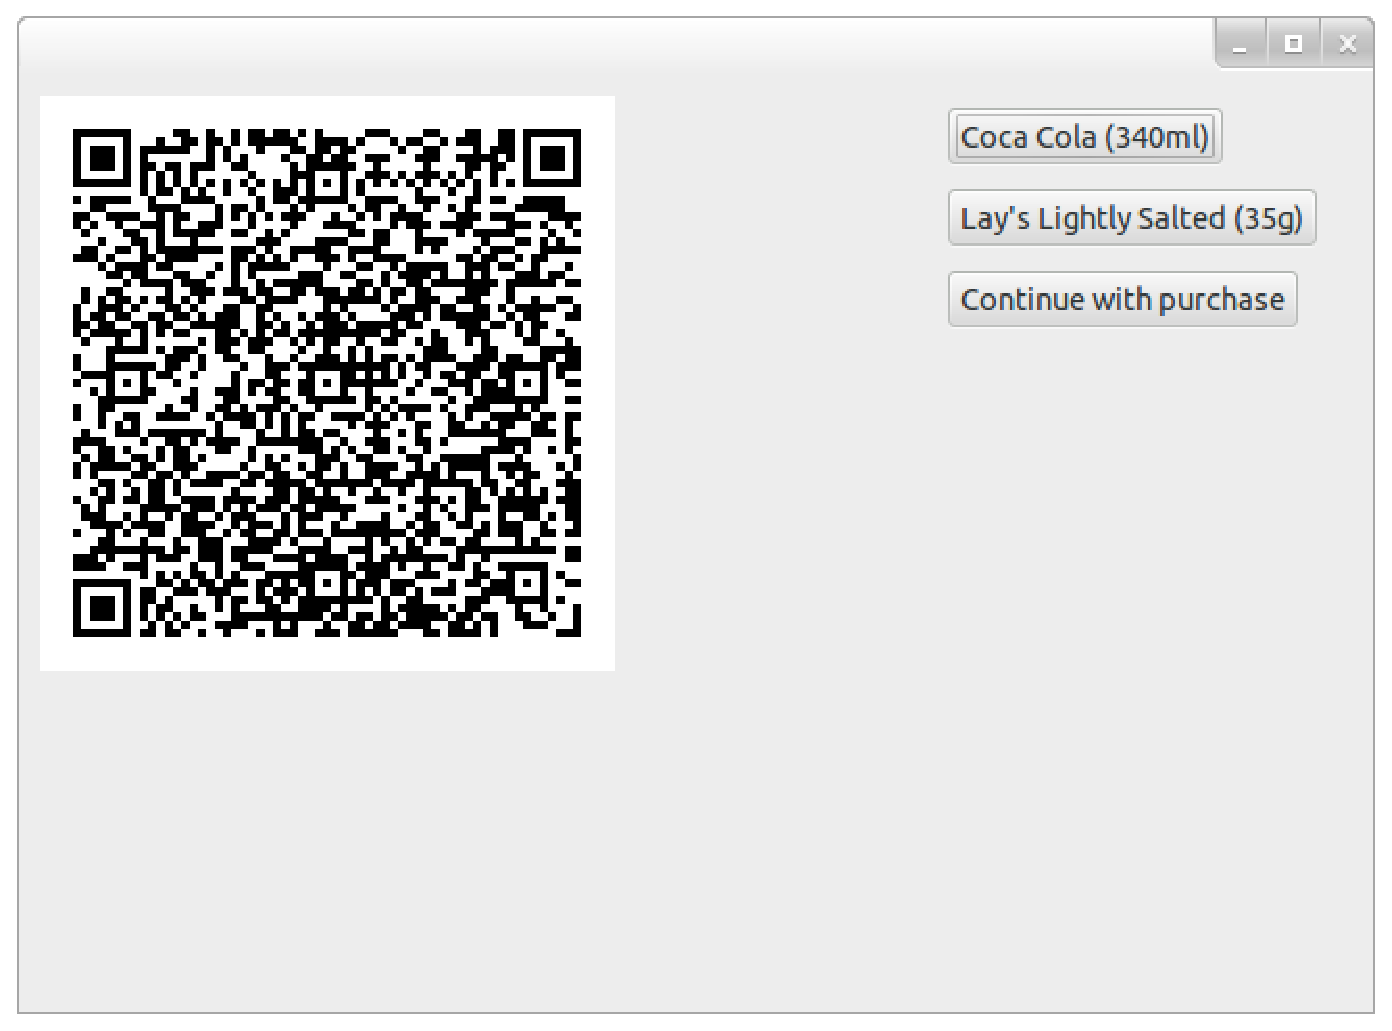
\includegraphics[scale=0.4]{gui_screenshot}
 \caption{A screenshot of the user interface}
 \label{fig:gui-screenshot}
\end{figure}

As can be seen from Figure \ref{fig:gui-processflow}, the GUI script is
responsible for calling the encryption script and the QR Code generation script.
It is also responsible for displaying the QR Code, to handle transactions from
the Android NFC app and to activate the correct motor inside the vending
machine. 

\subsection{Generate Product Code}

After the customer selects which product to buy from the GUI, the
encrypt\_elgamal script is called. This script is responsible for generating the
random hex character string, in accordance with the security scheme described in
Section \ref{sec:security-code-scheme}, encrypting, signing and encoding the
string in base 64 and embedding the random string inside a Uniform
Resource Locator (URL) that points to the web server. This URL is then sent to
the generate\_qrcode script described in Section \ref{sec:generate-qrcode}.

See Figure \ref{fig:gen-prod-code-processflow} for a detailed process flow
diagram.

\subsection{Generate QR Code}
\label{sec:gen-qrcode}

After the encrypt\_elgamal script has been run, the generate\_qrcode script is
called. This script is responsible for embedding the URL received from the
encrypt\_elgamal script into a QR Code. This is done by using a qrcode module
for Python called qrcode [\cite{website:qrcode-generator}].

\subsection{Read QR Code}

\subsection{NFC}

Because the Arduino version of this shield is locally available, and the cost issues related
to importing a NFC chip that is made for the Raspberry Pi, the Arduino version was bought for 
R780.00. Its Transistor-Transistor Logic (TTL) serial interface was configured in such a way
so that it can serially communicate with the Raspberry Pi's UART interface. It can be powered
by the 5V output pin from the Raspberry Pi. 

\subsection{qr code}

\section{Android app}
\label{sec:nfc-android-app}

\section{Motor and coil}
\label{sec:detail-switch}